\documentclass{beamer}
%\usetheme{Singapore}
\usepackage{tikz}
\usetikzlibrary{arrows,automata}

%\usepackage{pstricks,pst-node,pst-tree}
\usepackage{amssymb,latexsym}
\usepackage{graphicx}
\usepackage{fancyvrb}
\usepackage{hyperref}

\newcommand{\bi}{\begin{itemize}}
\newcommand{\ii}{\item}
\newcommand{\ei}{\end{itemize}}
\newcommand{\Show}[1]{\psshadowbox{#1}}

\newcommand{\set}[1]{\ensuremath{\{#1\}}}

\newcommand{\grf}[2]{\centerline{\includegraphics[width=#1\textwidth]{#2}}}
\newcommand{\tw}{\textwidth}
\newcommand{\bc}{\begin{columns}}
\newcommand{\ec}{\end{columns}}
\newcommand{\cc}[1]{\column{#1\textwidth}}

\newcommand{\bfr}[1]{\begin{frame}[fragile]\frametitle{{ #1 }}}
\newcommand{\efr}{\end{frame}}

\newcommand{\cola}[1]{\begin{columns}\begin{column}{#1\textwidth}}
\newcommand{\colb}[1]{\end{column}\begin{column}{#1\textwidth}}
\newcommand{\colc}{\end{column}\end{columns}}

\title{Introduction to Theory of Computation}
\author{Chapter 2}

\RecustomVerbatimEnvironment{Verbatim}{Verbatim}{frame=single}

\begin{document}
\begin{frame}
\maketitle

\end{frame}


\bfr{Find a DFA: 101 but not 111}
$
\{w : w \mbox{ contains the string 101 but not the string 111}\}
$

Start with the basics:
\pause
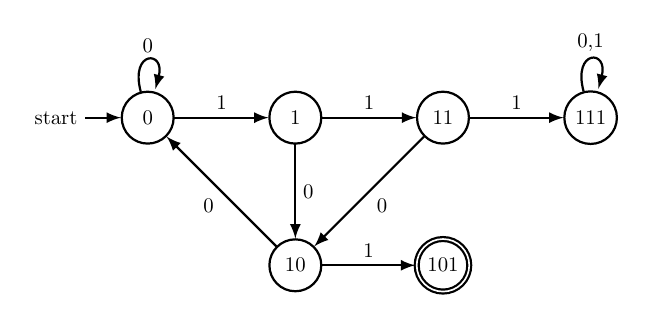
\begin{tikzpicture}[->,>=latex,thick,node distance=2.5cm,auto,every node/.style={scale=0.75}]
  \node[state,initial] (0) {0};
  \node[state] (1) [right of=0] {1};
  \node[state] (11) [right of=1] {11};
  \node[state] (111) [right of=11] {111};
  \node[state] (10) [below of=1] {10};
  \node[state,accepting] (101) [right of=10] {101};
  \path (0) edge [loop above] node {0} (0);
  \path (0) edge node {1} (1);
  \path (1) edge node {1} (11);
  \path (11) edge node {1} (111);
  \path (111) edge [loop above] node {0,1} (111);
  \path (11) edge node {0} (10);
  \path (10) edge node {0} (0);
  \path (1) edge node {0} (10);
  \path (10) edge node {1} (101);
\end{tikzpicture}

We know we can reject forever in state 111, but we cannot accept
forever in state 101 because we still have to make sure we don't get
a 111 later on.

\end{frame}

\bfr{Find a DFA: 101 but not 111}
$
\{w : w \mbox{ contains the string 101 but not the string 111}\}
$

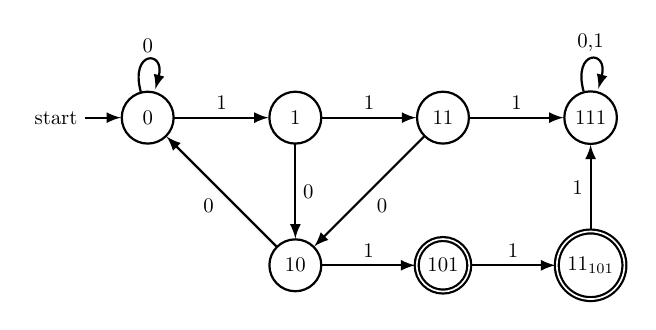
\begin{tikzpicture}[->,>=latex,thick,node distance=2.5cm,auto,every node/.style={scale=0.75}]
  \node[state,initial] (0) {0};
  \node[state] (1) [right of=0] {1};
  \node[state] (11) [right of=1] {11};
  \node[state] (111) [right of=11] {111};
  \node[state] (10) [below of=1] {10};
  \node[state,accepting] (101) [right of=10] {101};
  \node[state,accepting] (101+11) [right of = 101] {$11_{101}$};
  \path (0) edge [loop above] node {0} (0);
  \path (0) edge node {1} (1);
  \path (1) edge node {1} (11);
  \path (11) edge node {1} (111);
  \path (111) edge [loop above] node {0,1} (111);
  \path (11) edge node {0} (10);
  \path (10) edge node {0} (0);
  \path (1) edge node {0} (10);
  \path (10) edge node {1} (101);
  \path (101) edge node {1} (101+11);
  \path (101+11) edge node {1} (111);
\end{tikzpicture}

Now we just have to fill in the missing arcs.

\end{frame}


\bfr{Find a DFA: 101 but not 111}
$\{w : w \mbox{ contains the string 101 but not the string 111}\}$

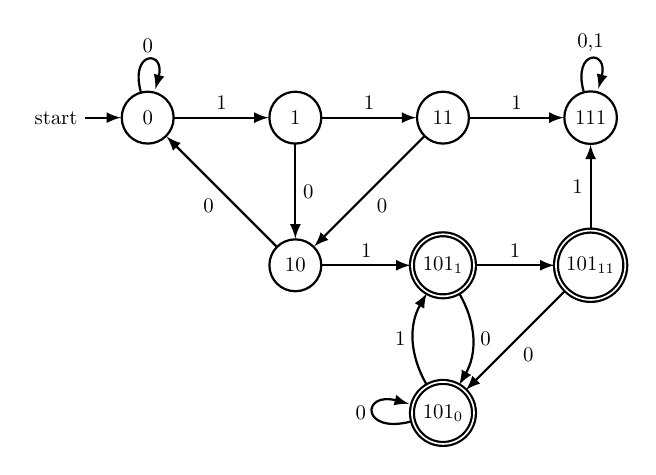
\begin{tikzpicture}[->,>=latex,thick,node distance=2.5cm,auto,every node/.style={scale=0.75}]
  \node[state,initial] (0) {0};
  \node[state] (1) [right of=0] {1};
  \node[state] (11) [right of=1] {11};
  \node[state] (111) [right of=11] {111};
  \node[state] (10) [below of=1] {10};
  \node[state,accepting] (101) [right of=10] {$101_{1}$};
  \node[state,accepting] (101+0) [below of=101] {$101_{0}$};
  \node[state,accepting] (101+11) [right of = 101] {${101}_{11}$};
  \path (0) edge [loop above] node {0} (0);
  \path (0) edge node {1} (1);
  \path (1) edge node {1} (11);
  \path (11) edge node {1} (111);
  \path (111) edge [loop above] node {0,1} (111);
  \path (11) edge node {0} (10);
  \path (10) edge node {0} (0);
  \path (1) edge node {0} (10);
  \path (10) edge node {1} (101);
  \path (101) edge node {1} (101+11);
  \path (101+11) edge node {1} (111);
  \path (101) edge [bend left] node {0} (101+0);
  \path (101+0) edge [bend left] node {1} (101);
  \path (101+0) edge [loop left] node {0} (101+0);
  \path (101+11) edge node {0} (101+0);
\end{tikzpicture}

\end{frame}


\bfr{Find a DFA: 101 but not 111, part 2}
$\{w : w \mbox{ contains the string 101 but not the string 111}\}$

Let's do the same thing by starting with the two base languages,
and forming the intersection.
\pause
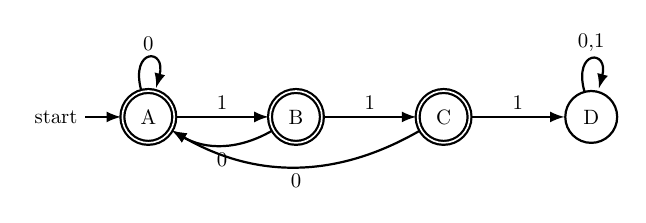
\begin{tikzpicture}[->,>=latex,thick,node distance=2.5cm,auto,every node/.style={scale=0.75}]
  \node[state,initial,accepting] (A) {A};
  \node[state,accepting] (B) [right of=A] {B};
  \node[state,accepting] (C) [right of=B] {C};
  \node[state] (D) [right of=C] {D};
  \path (A) edge [loop above] node {0} (A);
  \path (A) edge node {1} (B);
  \path (B) edge node {1} (C);
  \path (C) edge node {1} (D);
  \path (D) edge [loop above] node {0,1} (D);
  \path (B) edge [bend left] node {0} (A);
  \path (C) edge [bend left] node {0} (A);
\end{tikzpicture}

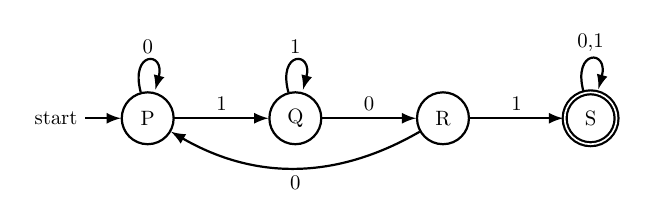
\begin{tikzpicture}[->,>=latex,thick,node distance=2.5cm,auto,every node/.style={scale=0.75}]
  \node[state,initial] (P) {P};
  \node[state] (Q) [right of=P] {Q};
  \node[state] (R) [right of=Q] {R};
  \node[state,accepting] (S) [right of=R] {S};
  \path (P) edge [loop above] node {0} (P);
  \path (P) edge node {1} (Q);
  \path (Q) edge node {0} (R);
  \path (R) edge node {1} (S);
  \path (S) edge [loop above] node {0,1} (S);
  \path (Q) edge [loop above] node {1} (Q);
  \path (R) edge [bend left] node {0} (P);
\end{tikzpicture}

\end{frame}

\bfr{Find a DFA: 101 but not 111, part 2}
$\{w : w \mbox{ contains the string 101 but not the string 111}\}$


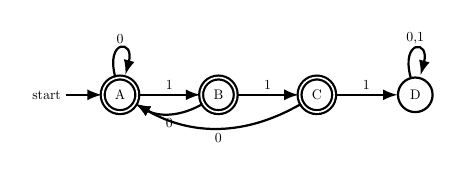
\begin{tikzpicture}[->,>=latex,thick,node distance=2.5cm,auto,every node/.style={scale=0.5}]
  \node[state,initial,accepting] (A) {A};
  \node[state,accepting] (B) [right of=A] {B};
  \node[state,accepting] (C) [right of=B] {C};
  \node[state] (D) [right of=C] {D};
  \path (A) edge [loop above] node {0} (A);
  \path (A) edge node {1} (B);
  \path (B) edge node {1} (C);
  \path (C) edge node {1} (D);
  \path (D) edge [loop above] node {0,1} (D);
  \path (B) edge [bend left] node {0} (A);
  \path (C) edge [bend left] node {0} (A);
\end{tikzpicture}
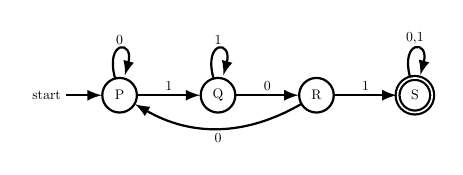
\begin{tikzpicture}[->,>=latex,thick,node distance=2.5cm,auto,every node/.style={scale=0.5}]
  \node[state,initial] (P) {P};
  \node[state] (Q) [right of=P] {Q};
  \node[state] (R) [right of=Q] {R};
  \node[state,accepting] (S) [right of=R] {S};
  \path (P) edge [loop above] node {0} (P);
  \path (P) edge node {1} (Q);
  \path (Q) edge node {0} (R);
  \path (R) edge node {1} (S);
  \path (S) edge [loop above] node {0,1} (S);
  \path (Q) edge [loop above] node {1} (Q);
  \path (R) edge [bend left] node {0} (P);
\end{tikzpicture}

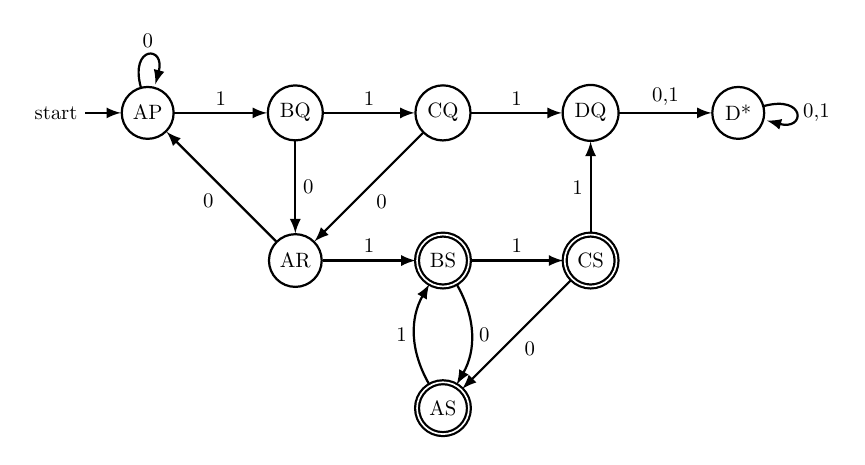
\begin{tikzpicture}[->,>=latex,thick,node distance=2.5cm,auto,every node/.style={scale=0.75}]
  \node[state,initial] (AP) {AP};
  \node[state] (BQ) [right of=AP] {BQ};
  \node[state] (CQ) [right of=BQ] {CQ};
  \node[state] (DQ) [right of=CQ] {DQ};
  \node[state] (D*) [right of=DQ] {D*};
  \node[state] (AR) [below of=BQ] {AR};
  \node[state,accepting] (BS) [right of=AR] {BS};
  \node[state,accepting] (CS) [right of=BS] {CS};
  \node[state,accepting] (AS) [below of=BS] {AS};
  \path (AP) edge [loop above] node {0} (AP);
  \path (AP) edge node {1} (BQ);
  \path (BQ) edge node {1} (CQ);
  \path (CQ) edge node {1} (DQ);
  \path (CQ) edge node {0} (AR);
  \path (DQ) edge node {0,1} (D*);
  \path (D*) edge [loop right] node {0,1} (D*);
  \path (BQ) edge node {0} (AR);
  \path (AR) edge node {0} (AP);
  \path (AR) edge node {1} (BS);
  \path (BS) edge node {1} (CS);
  \path (CS) edge node {1} (DQ);
  \path (BS) edge [bend left] node {0} (AS);
  \path (AS) edge [bend left] node {1} (BS);
  \path (CS) edge node {0} (AS);
\end{tikzpicture}
\end{frame}

\bfr{Union of Two DFAs}
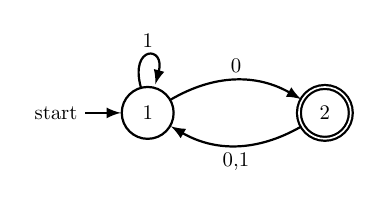
\begin{tikzpicture}[->,>=latex,thick,node distance=3cm,auto,every node/.style={scale=0.75}]
  \node[state,initial] (1) {1};
  \node[state,accepting] (2) [right of=1] {2};
  \path (1) edge [loop above] node {1} (1);
  \path (1) edge [bend left] node {0} (2);
  \path (2) edge [bend left] node {0,1} (1);
\end{tikzpicture}\hfill
\begin{tikzpicture}[->,>=latex,thick,node distance=3cm,auto,every node/.style={scale=0.75}]
  \node[state,initial] (3) {3};
  \node[state,accepting] (4) [right of=1] {4};
  \path (3) edge [loop above] node {0} (3);
  \path (3) edge [bend left] node {1} (4);
  \path (4) edge [bend left] node {0} (3);
  \path (4) edge [loop above] node{1} (3);
\end{tikzpicture}
\vfill\pause

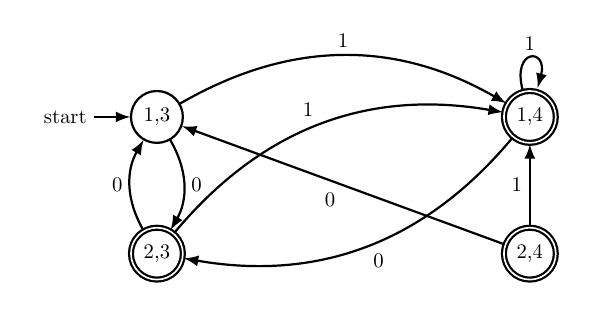
\begin{tikzpicture}[->,>=latex,thick,node distance=3cm,auto,every node/.style={scale=0.75}]
  \matrix[row sep=1cm,column sep=4cm]{
    \node[state,initial] (13) {1,3}; &
    \node[state,accepting] (14) {1,4}; \\
    \node[state,accepting] (23) {2,3}; &
    \node[state,accepting] (24) {2,4}; \\
  };
  \path (13) edge [bend left] node {0} (23);
  \path (13) edge [bend left] node {1} (14);
  \path (14) edge [bend left] node {0} (23);
  \path (14) edge [loop above] node {1} (14);
  \path (23) edge [bend left] node {0} (13);
  \path (23) edge [bend left] node {1} (14);
  \path (24) edge  node {0} (13);
  \path (24) edge  node {1} (14);
\end{tikzpicture}
\end{frame}


\bfr{Converting NFA to DFA, no $\epsilon$}
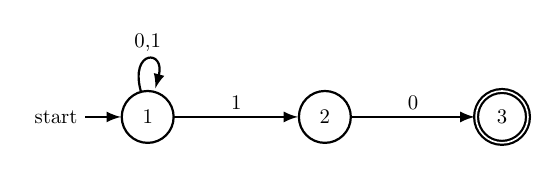
\begin{tikzpicture}[->,>=latex,thick,node distance=3cm,auto,every node/.style={scale=0.75}]
  \node[state,initial] (1) {1};
  \node[state] (2) [right of=1] {$2$};
  \node[state,accepting] (3) [right of=2] {$3$};
  \path (1) edge [loop above] node {0,1} (1);
  \path  (1) edge node {1} (2);
  \path (2) edge node {0} (3);
\end{tikzpicture}
\pause\hfill
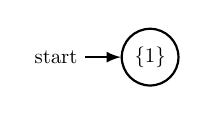
\begin{tikzpicture}[->,>=latex,thick,node distance=3cm,auto,every node/.style={scale=0.75}]
  \node[state,initial] (1) {\set{1}};
\end{tikzpicture}
\pause\vfill

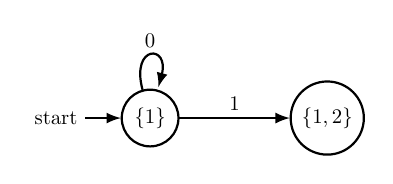
\begin{tikzpicture}[->,>=latex,thick,node distance=3cm,auto,every node/.style={scale=0.75}]
  \node[state,initial] (1) {\set{1}};
  \node[state] (12) [right of=1] {\set{1,2}};
  \path (1) edge [loop above] node {0} (1);
  \path (1) edge node {1} (12);
\end{tikzpicture}

\pause\vfill
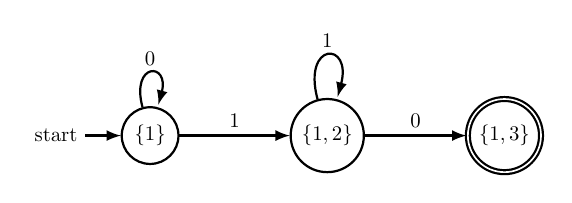
\begin{tikzpicture}[->,>=latex,thick,node distance=3cm,auto,every node/.style={scale=0.75}]
  \node[state,initial] (1) {\set{1}};
  \node[state] (12) [right of=1] {\set{1,2}};
  \node[state,accepting] (13) [right of=12] {\set{1,3}};
  \path (1) edge [loop above] node {0} (1);
  \path (1) edge node {1} (12);
  \path (12) edge [loop above] node {1} (12);
  \path (12) edge  node {0} (13);
\end{tikzpicture}

\pause\vfill
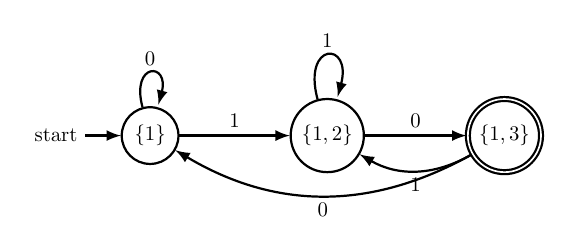
\begin{tikzpicture}[->,>=latex,thick,node distance=3cm,auto,every node/.style={scale=0.75}]
  \node[state,initial] (1) {\set{1}};
  \node[state] (12) [right of=1] {\set{1,2}};
  \node[state,accepting] (13) [right of=12] {\set{1,3}};
  \path (1) edge [loop above] node {0} (1);
  \path (1) edge node {1} (12);
  \path (12) edge [loop above] node {1} (12);
  \path (12) edge  node {0} (13);
  \path (13) edge [bend left] node {0} (1);
  \path (13) edge [bend left] node {1} (12);
\end{tikzpicture}

\end{frame}

\bfr{Converting NFA to DFA, with $\epsilon$-closure}
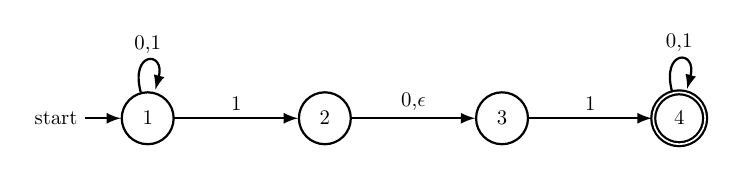
\begin{tikzpicture}[->,>=latex,thick,node distance=3cm,auto,every node/.style={scale=0.75}]
  \node[state,initial] (1) {$1$};
  \node[state] (2) [right of=1] {$2$};
  \node[state] (3) [right of=2] {$3$};
  \node[state,accepting] (4) [right of=3] {$4$};
  \path (1) edge [loop above] node {0,1} (1)
  (1) edge node {1} (2)
  (2) edge node {0,$\epsilon$} (3)
  (3) edge node {1} (4)
  (4) edge [loop above] node {0,1} (4);
\end{tikzpicture}
\vfill
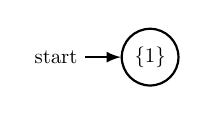
\begin{tikzpicture}[->,>=latex,thick,node distance=3cm,auto,every node/.style={scale=0.75}]
  \node[state,initial] (1) {$\{1\}$};
\end{tikzpicture}

\end{frame}

\bfr{Converting NFA to DFA, with $\epsilon$-closure}
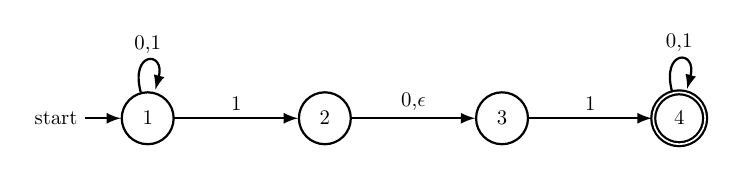
\begin{tikzpicture}[->,>=latex,thick,node distance=3cm,auto,every node/.style={scale=0.75}]
  \node[state,initial] (1) {$1$};
  \node[state] (2) [right of=1] {$2$};
  \node[state] (3) [right of=2] {$3$};
  \node[state,accepting] (4) [right of=3] {$4$};
  \path (1) edge [loop above] node {0,1} (1)
  (1) edge node {1} (2)
  (2) edge node {0,$\epsilon$} (3)
  (3) edge node {1} (4)
  (4) edge [loop above] node {0,1} (4);
\end{tikzpicture}
\vfill
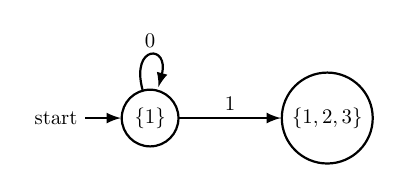
\begin{tikzpicture}[->,>=latex,thick,node distance=3cm,auto,every node/.style={scale=0.75}]
  \node[state,initial] (1) {$\{1\}$};
  \node[state] (123) [right of=1] {$\{1,2,3\}$};
  \path (1) edge [loop above] node {0} (1)
  (1) edge node {1} (123);
\end{tikzpicture}

\end{frame}

\bfr{Converting NFA to DFA, with $\epsilon$-closure}
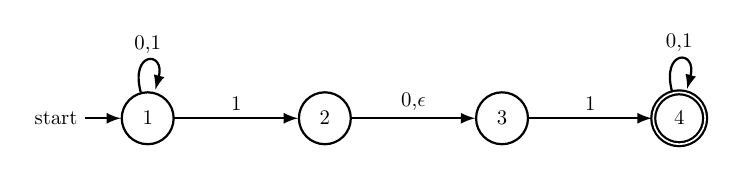
\begin{tikzpicture}[->,>=latex,thick,node distance=3cm,auto,every node/.style={scale=0.75}]
  \node[state,initial] (1) {$1$};
  \node[state] (2) [right of=1] {$2$};
  \node[state] (3) [right of=2] {$3$};
  \node[state,accepting] (4) [right of=3] {$4$};
  \path (1) edge [loop above] node {0,1} (1)
  (1) edge node {1} (2)
  (2) edge node {0,$\epsilon$} (3)
  (3) edge node {1} (4)
  (4) edge [loop above] node {0,1} (4);
\end{tikzpicture}
\vfill
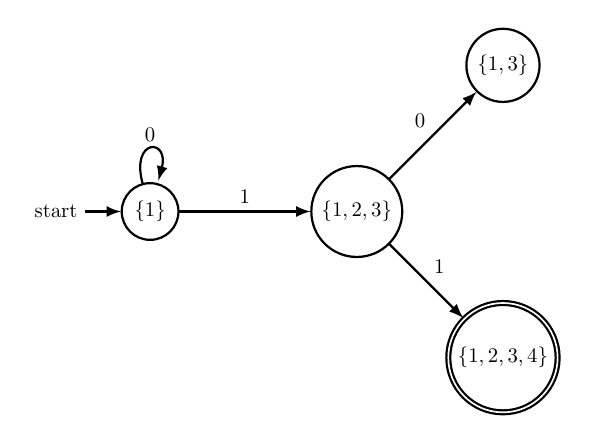
\begin{tikzpicture}[->,>=latex,thick,node distance=3.5cm,auto,every node/.style={scale=0.75}]
  \node[state,initial] (1) {$\{1\}$};
  \node[state] (123) [right of=1] {$\{1,2,3\}$};
  \node[state] (13) [above right of=123] {$\{1,3\}$};
  \node[state,accepting] (1234) [below right of=123] {$\{1,2,3,4\}$};
  \path (1) edge [loop above] node {0} (1)
  (1) edge node {1} (123)
  (123) edge node {0} (13)
  (123) edge node {1} (1234)
  ;
\end{tikzpicture}

\end{frame}

\bfr{Converting NFA to DFA, with $\epsilon$-closure}
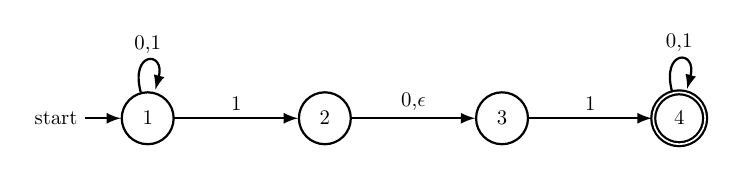
\begin{tikzpicture}[->,>=latex,thick,node distance=3cm,auto,every node/.style={scale=0.75}]
  \node[state,initial] (1) {$1$};
  \node[state] (2) [right of=1] {$2$};
  \node[state] (3) [right of=2] {$3$};
  \node[state,accepting] (4) [right of=3] {$4$};
  \path (1) edge [loop above] node {0,1} (1)
  (1) edge node {1} (2)
  (2) edge node {0,$\epsilon$} (3)
  (3) edge node {1} (4)
  (4) edge [loop above] node {0,1} (4);
\end{tikzpicture}
\vfill
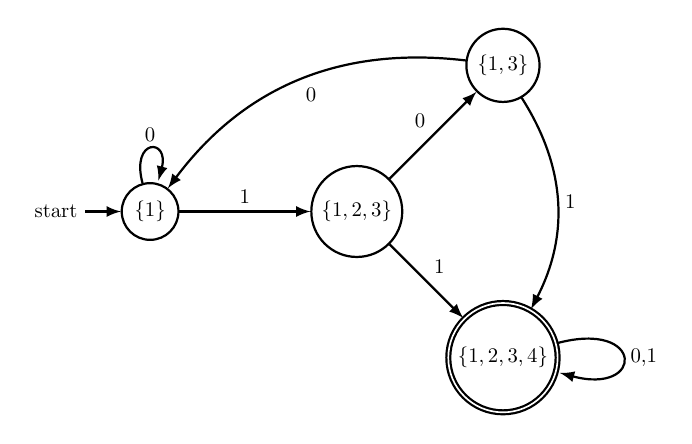
\begin{tikzpicture}[->,>=latex,thick,node distance=3.5cm,auto,every node/.style={scale=0.75}]
  \node[state,initial] (1) {$\{1\}$};
  \node[state] (123) [right of=1] {$\{1,2,3\}$};
  \node[state] (13) [above right of=123] {$\{1,3\}$};
  \node[state,accepting] (1234) [below right of=123] {$\{1,2,3,4\}$};
  \path (1) edge [loop above] node {0} (1)
  (1) edge node {1} (123)
  (123) edge node {0} (13)
  (123) edge node {1} (1234)
  (1234) edge [loop right] node {0,1} (1234)
  (13) edge [bend right] node {0} (1)
  (13) edge [bend left] node {1} (1234)
  ;
\end{tikzpicture}

\end{frame}

\bfr{Converting NFA to RE}
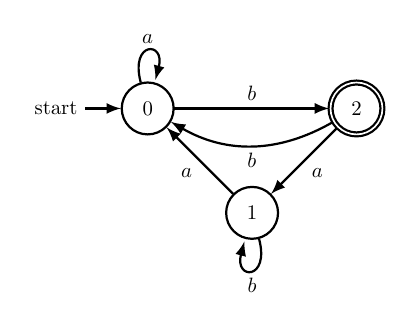
\begin{tikzpicture}[->,>=latex,thick,node distance=2.5cm,auto,every node/.style={scale=0.75}]
\node[initial,state] (0) {$0$};
\node[state] (1) [below right of=0] {$1$};
\node[state,accepting] (2) [above right of=1] {$2$};
\path (0) edge [loop above] node {$a$} (0)
      (0) edge  node {$b$} (2)
      (2) edge [bend left] node {$b$} (0)
      (1) edge [loop below] node {$b$} (1)
      (2) edge node {$a$} (1)
      (1) edge node {$a$} (0)
;
\end{tikzpicture}
\end{frame}

\bfr{Add new start and accept states}
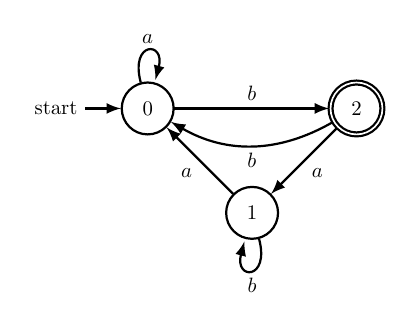
\begin{tikzpicture}[->,>=latex,thick,node distance=2.5cm,auto,every node/.style={scale=0.75}]
\node[initial,state] (0) {$0$};
\node[state] (1) [below right of=0] {$1$};
\node[state,accepting] (2) [above right of=1] {$2$};
\path (0) edge [loop above] node {$a$} (0)
      (0) edge  node {$b$} (2)
      (2) edge [bend left] node {$b$} (0)
      (1) edge [loop below] node {$b$} (1)
      (2) edge node {$a$} (1)
      (1) edge node {$a$} (0)
;
\end{tikzpicture}
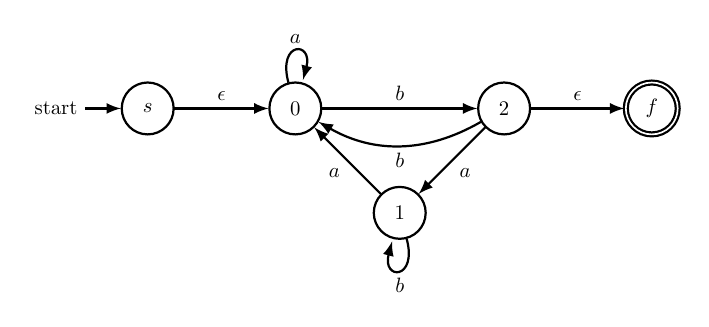
\begin{tikzpicture}[->,>=latex,thick,node distance=2.5cm,auto,every node/.style={scale=0.75}]
\node[initial,state] (s) {$s$};
\node[state] (0) [right of=s] {$0$};
\node[state] (1) [below right of=0] {$1$};
\node[state] (2) [above right of=1] {$2$};
\node[accepting,state] (f) [right of =2] {$f$};
\path (s) edge node {$\epsilon$} (0)
      (2) edge node {$\epsilon$} (f)
      (0) edge [loop above] node {$a$} (0)
      (0) edge  node {$b$} (2)
      (2) edge [bend left] node {$b$} (0)
      (1) edge [loop below] node {$b$} (1)
      (2) edge node {$a$} (1)
      (1) edge node {$a$} (0)
;
\end{tikzpicture}

\end{frame}

\bfr{Eliminate $2$}
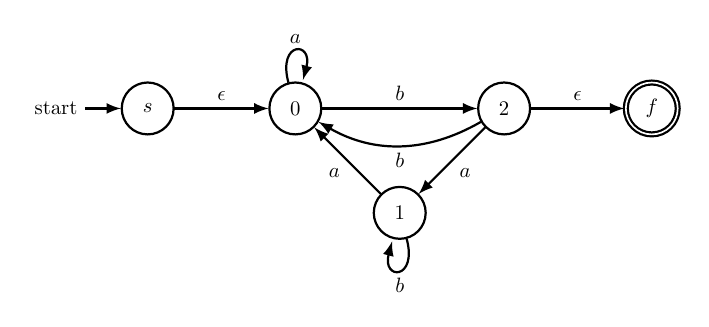
\begin{tikzpicture}[->,>=latex,thick,node distance=2.5cm,auto,every node/.style={scale=0.75}]
\node[initial,state] (s) {$s$};
\node[state] (0) [right of=s] {$0$};
\node[state] (1) [below right of=0] {$1$};
\node[state] (2) [above right of=1] {$2$};
\node[accepting,state] (f) [right of =2] {$f$};
\path (s) edge node {$\epsilon$} (0)
      (2) edge node {$\epsilon$} (f)
      (0) edge [loop above] node {$a$} (0)
      (0) edge  node {$b$} (2)
      (2) edge [bend left] node {$b$} (0)
      (1) edge [loop below] node {$b$} (1)
      (2) edge node {$a$} (1)
      (1) edge node {$a$} (0)
;
\end{tikzpicture}
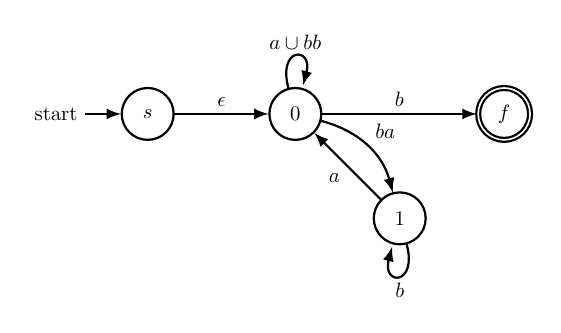
\begin{tikzpicture}[->,>=latex,thick,node distance=2.5cm,auto,every node/.style={scale=0.75}]
\node[initial,state] (s) {$s$};
\node[state] (0) [right of=s] {$0$};
\node[state] (1) [below right of=0] {$1$};
%\node[state] (2) [above right of=1] {$2$};
\node[accepting,state] (f) [above right of =1] {$f$};
\path (s) edge node {$\epsilon$} (0)
      (0) edge [loop above] node {$a\cup bb$} (0)
      (0) edge [bend left] node  {$ba$} (1)
      (0) edge  node {$b$} (f)
      (1) edge [loop below] node {$b$} (1)
      (1) edge node {$a$} (0)
;
\end{tikzpicture}
\end{frame}


\bfr{Eliminate $1$}
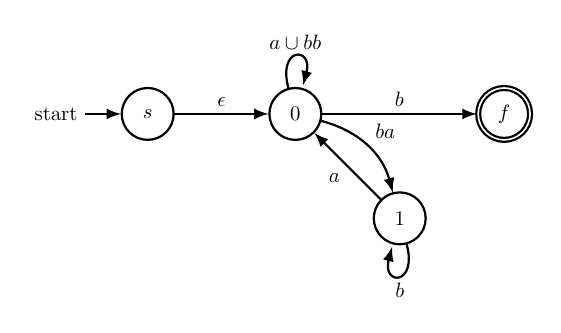
\begin{tikzpicture}[->,>=latex,thick,node distance=2.5cm,auto,every node/.style={scale=0.75}]
\node[initial,state] (s) {$s$};
\node[state] (0) [right of=s] {$0$};
\node[state] (1) [below right of=0] {$1$};
%\node[state] (2) [above right of=1] {$2$};
\node[accepting,state] (f) [above right of =1] {$f$};
\path (s) edge node {$\epsilon$} (0)
      (0) edge [loop above] node {$a\cup bb$} (0)
      (0) edge [bend left] node  {$ba$} (1)
      (0) edge  node {$b$} (f)
      (1) edge [loop below] node {$b$} (1)
      (1) edge node {$a$} (0)
;
\end{tikzpicture}
\begin{tikzpicture}[->,>=latex,thick,node distance=2.5cm,auto,every node/.style={scale=0.75}]
\node[initial,state] (s) {$s$};
\node[state] (0) [right of=s] {$0$};
%\node[state] (1) [below right of=0] {$1$};
%\node[state] (2) [above right of=1] {$2$};
\node[accepting,state] (f) [above right of =1] {$f$};
\path (s) edge node {$\epsilon$} (0)
      (0) edge [loop above] node {$a\cup bb\cup bab^*a$} (0)
      (0) edge  node {$b$} (f)
;
\end{tikzpicture}

\end{frame}

\bfr{Eliminate $0$}

\begin{tikzpicture}[->,>=latex,thick,node distance=2.5cm,auto,every node/.style={scale=0.75}]
\node[initial,state] (s) {$s$};
\node[state] (0) [right of=s] {$0$};
%\node[state] (1) [below right of=0] {$1$};
%\node[state] (2) [above right of=1] {$2$};
\node[accepting,state] (f) [above right of =1] {$f$};
\path (s) edge node {$\epsilon$} (0)
      (0) edge [loop above] node {$a\cup bb\cup bab^*a$} (0)
      (0) edge  node {$b$} (f)
;
\end{tikzpicture}

\bigskip

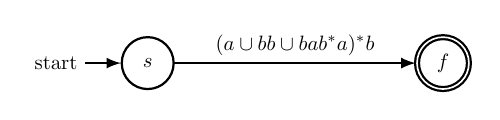
\begin{tikzpicture}[->,>=latex,thick,node distance=5cm,auto,every node/.style={scale=0.75}]
\node[initial,state] (s) {$s$};
%\node[state] (0) [right of=s] {$0$};
%\node[state] (1) [below right of=0] {$1$};
%\node[state] (2) [above right of=1] {$2$};
\node[accepting,state] (f) [right of=s] {$f$};
\path (s) edge  node {$(a\cup bb\cup bab^*a)^*b$} (f)
;
\end{tikzpicture}

\end{frame}

\end{document}
